% Modeled after the following
% A simple Tree
% Author: Stefan Kottwitz
% https://www.packtpub.com/hardware-and-creative/latex-cookbook
\documentclass[border=10pt]{standalone}
\usepackage{tikz}
\begin{document}
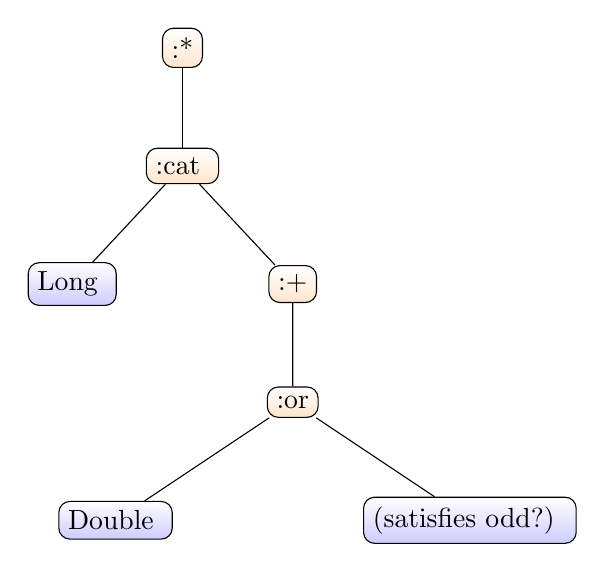
\begin{tikzpicture}[sibling distance=10em,
  every node/.style = {shape=rectangle, rounded corners,
    draw, align=center,
    top color=white, bottom color=orange!20}]]
    \tikzstyle{level 2}=[sibling distance=28mm]
    \tikzstyle{level 4}=[sibling distance=45mm]
  \node {\code{:*}}
  child { node { \code{:cat} } 
    child { node [bottom color=blue!20] {\code{Long} } }
    child { node {\code{:+}} 
      child { node {\code{:or}}
        child { node [bottom color=blue!20] {\code{Double} } }
        child { node [bottom color=blue!20] {\code{(satisfies odd?)} } } } } } ;
\end{tikzpicture}
\end{document}
